\documentclass[11pt,final]{amsart}
\usepackage[margin=1in]{geometry}
\usepackage{fancyvrb}

\DefineShortVerb{\|} % this changes the meaning of the | character.

\newcommand{\PISMREV}{\input{revision.tex}}
\newcommand{\PETSCREL}{2.3.3-p2}

%\addtolength\topmargin{-.1in}
\addtolength\textheight{0.1in}
\addtolength{\oddsidemargin}{-.4in}
\addtolength{\evensidemargin}{-.4in}
\addtolength{\textwidth}{0.9in}
\newcommand{\normalspacing}{\renewcommand{\baselinestretch}{1.1}\tiny\normalsize}
\newcommand{\tablespacing}{\renewcommand{\baselinestretch}{1.0}\tiny\normalsize}
\normalspacing

\usepackage{bm,url,xspace,verbatim}
\usepackage{amssymb,amsmath}
\usepackage[final,pdftex]{graphicx}
\usepackage[pdftex]{hyperref}

%% uncomment to see locations of index entries
%\usepackage{showidx}

\newcommand{\ddt}[1]{\ensuremath{\frac{\partial #1}{\partial t}}}
\newcommand{\ddx}[1]{\ensuremath{\frac{\partial #1}{\partial x}}}
\newcommand{\ddy}[1]{\ensuremath{\frac{\partial #1}{\partial y}}}
\renewcommand{\t}[1]{\texttt{#1}}
\newcommand{\Matlab}{\textsc{Matlab}\xspace}
\newcommand{\bq}{\mathbf{q}}
\newcommand{\bU}{\mathbf{U}}
\newcommand{\eps}{\epsilon}
\newcommand{\grad}{\nabla}
\newcommand{\Div}{\nabla\cdot}

%% macros having to do with documentation for options; note these appear in the index
\newcommand{\und}{\_\!\_}

%\newcommand{\alphaoptionindex}[1]{\index{alphabetical list of options for PISM (and PETSc)!\texttt{-#1}}}
\newcommand{\pismoptionindex}[1]{\index{options for PISM (and PETSc)!\texttt{-#1}}}
\newcommand{\intextoption}[1]{\texttt{-#1}\pismoptionindex{#1}}

%\newcommand{\rawopt}[1]{\vspace{1mm}\noindent \large\texttt{-#1}\normalsize\pismoptionindex{#1}\alphaoptionindex{#1}}
\newcommand{\rawopt}[1]{\vspace{1mm}\noindent \Large\texttt{-#1}\normalsize\pismoptionindex{#1}}
\newcommand{\opt}[1]{\rawopt{#1}\,:\quad}
\newcommand{\optdef}[2]{\rawopt{#1}\,[\textsl{#2}]:\quad}
\newcommand{\optrestrict}[2]{\rawopt{#1}\,[\texttt{#2} \textsl{only}]:\quad}
\newcommand{\optdefrestrict}[3]{\rawopt{#1}\,[\textsl{#2}]\,[\texttt{#3} \textsl{only}]:\quad}


% preamble:

\makeindex

\title[PISM Installation Manual]{\protect{\Large \emph{PISM}, a Parallel Ice
    Sheet Model:\normalsize} \\ \protect{\Large \bigskip \bigskip Installation
    Manual\normalsize}}

\author[]{Ed Bueler \\ Constantine Khroulev}

\date{\today. \href{mailto:help@pism-docs.org}{help@pism-docs.org}. Based on
  PISM rev \PISMREV\,and PETSC rel \PETSCREL. \\ Get PISM development version
  by ``\quad\texttt{svn co http://svn.gna.org/svn/pism/trunk pism-dev}\quad''}

\pdfinfo{
/Title (PISM Installation Manual)
/Author (Constantine Khroulev and Ed Bueler)
/Subject (Downloading and installing PISM, a Parallel Ice-Sheet Model)
/Keywords (PISM ice-sheet modeling installation)
}

\sloppy

\begin{document}
\maketitle
\thispagestyle{empty}

\vspace{2.0in}
\begin{center}
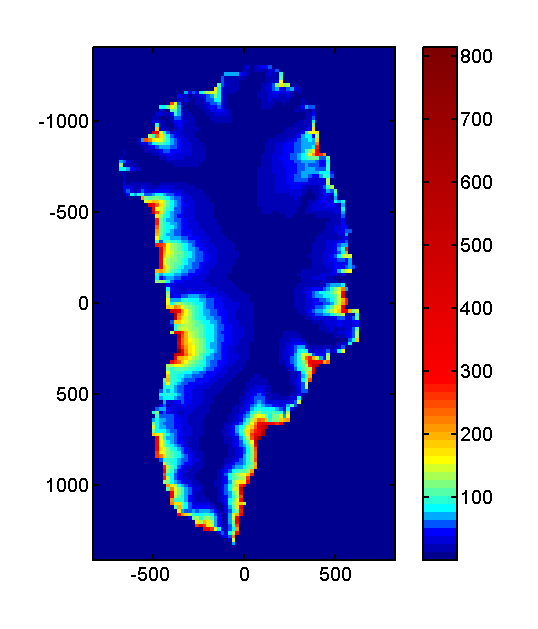
\includegraphics[width=2.5in,keepaspectratio=true]{figs/greencbar_SSL2}\, 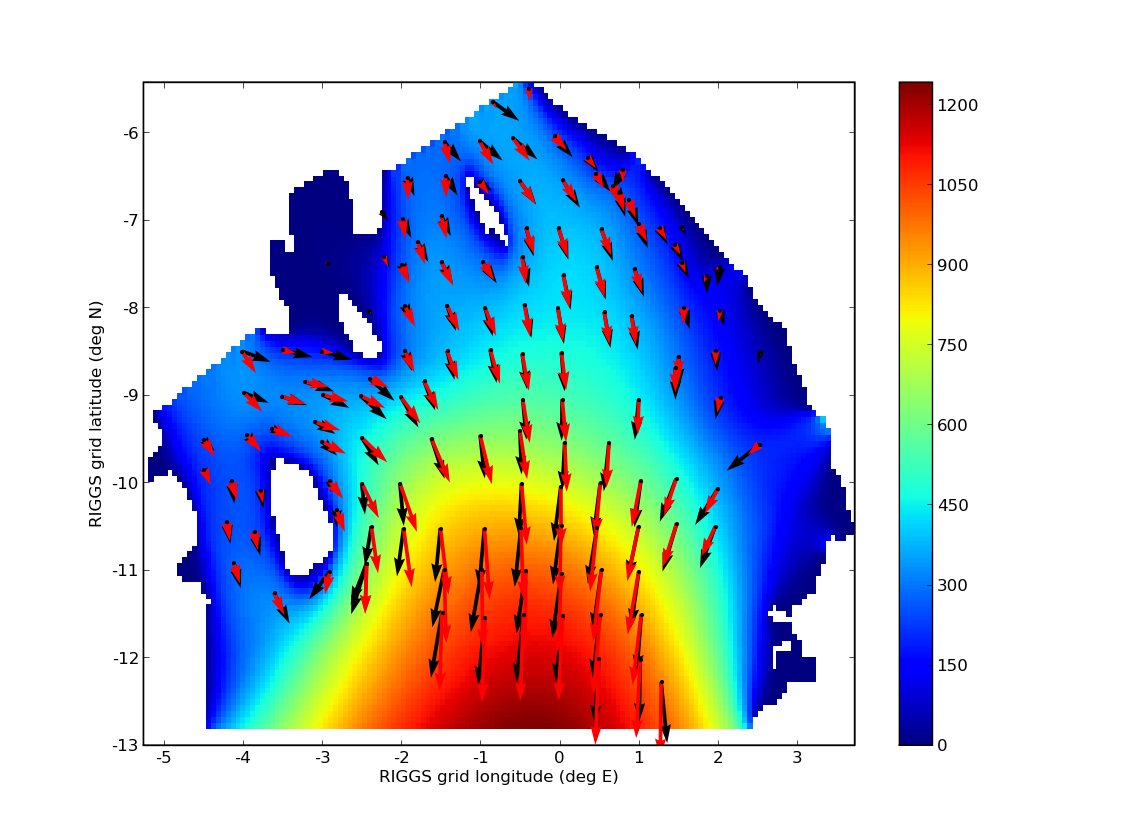
\includegraphics[width=3.2in,keepaspectratio=true]{figs/rossquiver}
\end{center}

\newpage
\phantom{bob}
\vspace{1in}
\begin{quote}
\textsl{Copyright (C) 2004--2008 Ed Bueler and Constantine Khroulev}
\medskip

\noindent \textsl{This file is part of PISM.}
\medskip

\noindent \textsl{PISM is free software; you can redistribute it and/or modify it under the terms of the GNU General Public
  License as published by the Free Software Foundation; either version 2 of the License, or (at your option) any later version.}
\medskip

\noindent \textsl{PISM is distributed in the hope that it will be useful, but WITHOUT ANY WARRANTY; without even the implied
  warranty of MERCHANTABILITY or FITNESS FOR A PARTICULAR PURPOSE. See the GNU General Public License for more details.} \medskip

\noindent \textsl{You should have received a copy of the GNU General Public License\index{GPL (\emph{GNU Public License})} along
  with PISM; see \emph{\texttt{COPYING}} in PISM root directory. If not, write to the Free Software Foundation, Inc., 51 Franklin
  St, Fifth Floor, Boston, MA 02110-1301 USA}
\end{quote}
\vspace{1in}
\normalspacing

\newpage
\setcounter{tocdepth}{2}
\tableofcontents


\newpage
\section{Introduction}\label{sect:intro}

This \emph{Installation Manual} describes how to download the PISM source code and install PISM and the libraries it needs.

Information about PISM is online at
\begin{center}
  \href{http://www.pism-docs.org}{\t{www.pism-docs.org}}
\end{center}

\begin{center}
\large
 \emph{WARNING}:\index{PISM!warning}  PISM is an ongoing project.  Ice sheet modeling is complicated and not mature (in 2008, anyway).  Please don't trust the results of PISM or any other ice sheet model without a fair amount of exploration.  Also, please don't expect all your questions to be answered here.  Write to us with questions: \large
\bigskip

\href{mailto:help@pism-docs.org}{\texttt{help@pism-docs.org}}
\normalsize
\end{center}

\clearpage
\section{Prerequisites}
\label{sec:prerequisites}

The following table lists the dependencies for PISM, arranged alphabetically. These are needed to build a fully-functional PISM from
source and do all the examples in the \emph{User's Manual}.
\bigskip
\begin{center}
\begin{tabular*}{1.0\linewidth}{lllp{0.25\linewidth}}\hline
  \textbf{Library/Program} & \textbf{Site} & \textbf{Required?} & \textbf{Comment} \\
  FFTW & \href{http://www.fftw.org/}{\t{www.fftw.org}} & \emph{recommended} & needed for earth deformation; if not present set |WITH_FFTW=0|\\
  GSL & \href{http://www.gnu.org/software/gsl/}{\t{www.gnu.org/software/gsl}} & \emph{required} &  \\
  |matplotlib| & \href{http://matplotlib.sourceforge.net/}{\t{matplotlib.sourceforge.net}} & \emph{recommended} & used in Python scripts \\
  MPI & \href{http://www-unix.mcs.anl.gov/mpi/}{\t{www-unix.mcs.anl.gov/mpi}} & \emph{required} & \\
  NetCDF & \href{http://www.unidata.ucar.edu/software/netcdf/}{\t{www.unidata.ucar.edu/software/netcdf}}\small & \emph{required} & \\
  |netcdf4-python| & \href{http://code.google.com/p/netcdf4-python/}{\t{code.google.com/p/netcdf4-python}}\small & \emph{recommended}  & used in Python scripts  \\  \texttt{numpy} & \href{http://numpy.scipy.org/}{\t{numpy.scipy.org}} & \emph{recommended}  & used in Python scripts  \\
  PETSc &  \href{http://www-unix.mcs.anl.gov/petsc/petsc-as/}{\t{www-unix.mcs.anl.gov/petsc}} & \emph{required} & version $\ge$ \PETSCREL \\
  Python & \href{http://python.org/}{\t{python.org}} & \emph{required} & required for PETSc configuration and scripts used in the \emph{User's Manual}\\
  |scikits.delaunay| & \href{http://scipy.org/scipy/scikits}{\t{scipy.org/scipy/scikits}} & \emph{recommended} & used in Python scripts \\
  Subversion & \href{http://subversion.tigris.org/}{\t{subversion.tigris.org}} & \emph{required} & \\ 
  \hline
\end{tabular*}
\end{center}

\newpage
\section{Generic installation instructions}\label{sect:generic}

\subsection{Installing prerequisities}
\renewcommand{\labelenumi}{\textbf{\arabic{enumi}.}~}
\begin{enumerate}
\item You will need a UNIX system with internet access. A GNU/Linux environment will be easiest but other UNIX versions have been
  used successfully. Package management systems are useful for installing many of the tools listed in section
  \ref{sec:prerequisites}, \emph{but} an up-to-date PETSc distribution may not be available in your system's package
  repositories. You will need \href{http://www.python.org/}{Python} and \href{http://subversion.tigris.org/}{Subversion}
  installed, but these are included in all current Linux distributions. To use the (recommended) graphical output of PISM you will
  need an \href{http://www.x.org/}{X Windows server}.

\item As PISM is currently under rapid development, we distribute it only as compilable source code. On the other hand, there are
  several software libraries needed by PISM. Therefore the ``header files'' for these libraries are required for building PISM. In
  particular this means that the ``developer's versions'' of the libraries are needed if the libraries are downloaded from package
  repositories like Debian.

\item PISM uses \href{http://www.unidata.ucar.edu/software/netcdf/}{NetCDF (= \emph{network Common Data Form})}\index{NetCDF} for
  an input and output file format. If it is not already present, install it using the instructions at the webpage or using a
  package management system.

\item PISM uses the \href{http://www.gnu.org/software/gsl/}{GSL (= \emph{GNU Scientific Library})}\index{GSL (\emph{GNU Scientific
      Library})} for certain numerical calculations and special functions. If it is not already present, install it using the
  instructions at the webpage or using a package management system.

\item PISM optionally uses the \href{http://www.fftw.org/}{``FFTW'' library (FFTW = \emph{Fastest Fourier Transform in the
      West})}\index{FFTW (\emph{Fastest Fourier Transform in the West})} in approximating the deformation of the solid earth under
  ice loads \cite{BLKfastearth}. If you want the functionality of this earth model, which is coupled to the ice flow and which we
  recommend, install FFTW or check that it is installed already. If FFTW is \emph{not installed}, however, turn off PISM's attempt
  to build with it by setting the environment variable |WITH_FFTW=0|. If this library is absent, all of PISM will work
  \emph{except} for the bed deformation model described in the paper \cite{BLKfastearth}.

\item You will need a version of \href{http://www-unix.mcs.anl.gov/mpi/}{MPI (= \emph{Message Passing Interface})}.\index{MPI
    (\emph{Message Passing Interface})} Your system may have an existing MPI installation, in which case the path to the MPI
  directory will be used when installing PETSc below. Otherwise we recommend that you allow PETSc to download
  \href{http://www-unix.mcs.anl.gov/mpi/mpich2/}{MPICH2} as part of the PETSc configure process (next). In either case, once MPI
  is installed, you will want to add the MPI |bin| directory to your path so that you can invoke MPI using the |mpiexec|
  or |mpirun| command. For example, you can add it with the statement

\verb|export PATH=/home/user/mympi/bin:$PATH|  \qquad (for |bash| shell)

\noindent or

\verb|setenv PATH /home/user/mympi/bin:$PATH|  \qquad (for |csh| or |tcsh| shell).

\noindent Such a statement can, of course, appear in your |.bashrc|, |.profile|, or |.cshrc| file so that there is
no need to retype it each time you use MPI.

\medskip
\begin{center}
  \emph{From now on this manual will assume the use of} bash.
\end{center}
\medskip

\item PISM uses \href{http://www-unix.mcs.anl.gov/petsc/petsc-2/index.html}{PETSc (= \emph{Portable Extensible Toolkit for
      Scientific Computation})}.\index{PETSc (\emph{Portable Extensible Toolkit for Scientific computation})} As mentions of this
  library will occur frequently in this manual, note ``PETSc'' is pronounced ``pet-see''. Download the PETSc source by grabbing
  the current gzipped tarball at
   \begin{center}
    \href{http://www-unix.mcs.anl.gov/petsc/petsc-as/download/index.html}{\t{www-unix.mcs.anl.gov/petsc/petsc-as/download/index.html}}
  \end{center}
  PISM requires a version of PETSc which is \texttt{\PETSCREL} or later. The ``lite'' form of PETSc is fine if you are willing to
  depend on an internet connection for accessing the PETSc documentation.

  You should configure and build PETSc \emph{essentially} as described on the
  \href{http://www-unix.mcs.anl.gov/petsc/petsc-2/documentation/installation.html}{PETSc installation page}, but it might be best
  to read the following comments on the PETSc configure and build process first:

\renewcommand{\labelenumii}{(\roman{enumii})}\begin{enumerate}
\item Untar in your preferred location, but note PETSc should \emph{not} be configured (next) using root privileges. Note that you
  will need to define the environment variable |PETSC_DIR|\index{PETSC\und DIR} before configuring PETSc (next). For instance,
  once you have entered the PETSc directory just untarred, \verb|export PETSC_DIR=$PWD|. (Or \verb|PETSC_DIR=`pwd`|. In this case,
  note the use of the backprime (\emph{accent-grave}) character, and not the single apostrophe |'|.)

\item When you run the configure script in the PETSc directory, the following options are recommended; note PISM uses shared
  libraries by default:\index{PETSC\und ARCH}
\begin{verbatim}
$  export PETSC_ARCH=linux-gnu-cxx
$  ./config/configure.py --with-shared --with-c-support \
   --with-clanguage=cxx --with-debugging=no
\end{verbatim}

Turning off the inclusion of the debugging symbols gives a significant speed improvement.

Note that there is no PISM use of Fortran, and that it is sometimes convenient to have PETSc grab a local copy of BLAS\index{BLAS (\emph{Basic Linear Algebra Subsystem})} and LAPACK\index{LAPACK (\emph{Linear Algebra PACKage})} rather than using the system-wide version.  So one may add ``\verb|--with-fortran=0| \verb|--download-c-blas-lapack=1|'' to the other configure options.

\item If there is an existing MPI\index{MPI (\emph{Message Passing Interface})} installation, for example at \verb|/home/user/mympi/|, one can point PETSc to it by adding the option \verb|--with-mpi-dir=/home/user/mympi/|.  The path used in this option must have MPI executables \verb|mpicxx| and \verb|mpicc|, and either \verb|mpiexec| or \verb|mpirun|, in subdirectory \verb|bin/| and MPI library files in subdirectory \verb|lib/|.

\item On the other hand, it seems common that one needs to tell PETSc to download MPI\index{MPI (\emph{Message Passing Interface})} into a place it understands, even if there is an existing MPI.  If you get messages suggesting that PETSc cannot configure using your existing MPI, you might try \verb|configure.py| with option \verb|--download-mpich=1|.

\item Configuration of PETSc for a batch system requires special procedures described at the PETSc documentation site.  One starts with a configure option \verb|--with-batch=1|.  See the ``Installing on machine requiring cross compiler or a job scheduler'' section of the \href{http://www-unix.mcs.anl.gov/petsc/petsc-2/documentation/installation.html}{PETSc installation page}.

\item  Configuring PETSc takes many minutes even when everything goes smoothly.   A value for the environment variable \verb|PETSC_ARCH| will be reported at the end of the configure process; take note of this value.  (Note that a previously installed PETSc can be reconfigured with a new \verb|PETSC_ARCH| if necessary.)

\item  After \verb|configure.py| finishes, you will need to \verb|make all test| in the PETSc directory and watch the result.  If the X Windows system is functional some example viewers will appear; as noted you will need the X header files for this to work.

\item Finally, you will want to set the \verb|PETSC_DIR| and the \verb|PETSC_ARCH| environment variables in your \verb|.profile| or \verb|.bashrc| file.  Also remember to add the MPI \verb|bin| directory to your \verb|PATH|.  For instance, if you used the option \verb|--download-mpich=1| in the PETSc configure, the MPI \verb|bin| directory will have a path like \verb|$PETSC_DIR/| \verb|externalpackages/mpich2-1.0.4p1/$PETSC_ARCH/bin/|.  Therefore the lines 
\begin{verbatim}
export PETSC_DIR=/home/user/petsc-2.3.3-p2/
export PETSC_ARCH=linux-gnu-cxx
export PATH=$PETSC_DIR/externalpackages/mpich2-1.0.4p1/$PETSC_ARCH/bin/:$PATH
\end{verbatim}
\noindent could appear in one of those files.
\end{enumerate}
\end{enumerate}
\medskip See the table in the section \ref{sec:prerequisites} for a summary of the dependencies on external libraries, including
those mentioned so far.

\subsection{Installing PISM itself}
\label{sec:pism-itself}
At this point you have configured the environment which PISM needs.  You are ready to build PISM itself, which is a much quicker procedure!

\begin{enumerate}\setcounter{enumi}{7}
\item Get the latest source\index{PISM!download source code} for PISM using the Subversion\index{Subversion} version control system:
\begin{enumerate}
\item \label{getPISMstep} Check the website \url{http://www.pism-docs.org/} for the latest version of PISM.
\item Do
\begin{verbatim}
$  svn co http://svn.gna.org/svn/pism/trunk pism-dev
\end{verbatim}
\item A directory called ``\verb|pism-dev/|'' will be created.  Note that in the future when you enter that directory, \verb|svn update| will update to the latest revision of PISM.\footnote{Of course, after \t{svn update} you will \t{make} and \t{make install} to recompile and relink PISM. Alternatively, you can \t{make update}, which will run \t{svn update} and then rebuild PISM if necessary.}
\end{enumerate}

\item Build PISM:\footnote{Please report any problems you meet at this build stage by sending us the output: \href{mailto:help@pism-docs.org}{help@pism-docs.org}.}
\begin{verbatim}
$  cd pism-dev
$  make
$  make install
\end{verbatim}
\noindent  Note that the ``\verb|make install|'' puts executables, including \verb|pismd|,\index{pismd} \verb|pismr|,\index{pismr} \verb|pismv|,\index{pismv} and \verb|pisms|,\index{pisms} in the \verb|pism-dev/bin/| subdirectory. Object files created during the build process (located in the \verb|build| subdirectory) are not deleted by the \verb|install| target, so please do ``\verb|make clean|'' if space is an issue. Note ``\verb|make install|'' does not require root permission as it only writes to the local \verb|pism-dev/bin| and \verb|pism-dev/lib|.

\item PISM executables can be run most easily by adding the directories \verb|pism-dev/bin/| and \verb|pism-dev/util/| to your \verb|PATH|.  The former directory contains the major PISM executables while the latter contains several useful scripts.  For instance, this command can be done in the \verb|bash| shell or in your \verb|.bashrc| file:\index{setting the \$PATH to find PISM executables}
\begin{verbatim}
export PATH=/home/user/pism-dev/bin:/home/user/pism-dev/util:$PATH
\end{verbatim}
\end{enumerate}


\subsection{Installing Python packages}
\label{sec:recommended}

If you're lucky, you might be able to install all the Python packages mentioned in section \ref{sec:prerequisites} using a package
manager. On the other hand, |netcdf4-python| and |scikits.delaunay| are not currently available in Debian package repositories and
are easy to install using Python setuptools (included with recent versions of Python).

If you are using NetCDF 3.6.2, you can install |netcdf4-python| by downloading a tarball from
\href{http://code.google.com/p/netcdf4-python/}{the project homepage}. After entering the directory you just untarred, run
\begin{verbatim}
$  sudo NETCDF3_DIR=/usr/ python setup-nc3.py install
\end{verbatim}
assuming that NetCDF was installed in the |/usr/| tree. And if you use NetCDF 4.0, do
\begin{verbatim}
$  sudo NETCDF4_DIR=/usr/ HDF5_DIR=/usr/ python setup.py install
\end{verbatim}
(again, assuming that HDF5 and NetCDF were installed in the |/usr/| tree.

\bigskip
Installing |scikits.delaunay| can be accomplished by running
\begin{verbatim}
$  svn co http://svn.scipy.org/svn/scikits/trunk/delaunay
$  cd delaunay; sudo python setup.py install
\end{verbatim}

\clearpage
\section{Installing PISM on a Debian-based Linux system}
\label{sec:debian}
It is now possible to install all the PISM prerequisites on a Debian-based system (such as Ubuntu) using a package manager.

\begin{enumerate}
\item You will need to find and install (using |synaptic|, for example) the following packages:
  \begin{center}
    \begin{tabular*}{0.9\linewidth}{p{0.15\linewidth}p{0.7\linewidth}}
      \hline
      Package name & Comments\\
      |petsc-dev| & depends on |libpetsc2.3.3-dev|; this package 
      depends on |libpetsc2.3.3|, |libopenmpi-dev|, |libx11-dev|,
      |libblas-dev|, |liblapack-dev|, |gfortran|, and others; 
      note |libopenmpi-dev| depends on |libopenmpi1| and
      replaces openmpi-bin\\
      |libgsl0-dev| & \\
      |libfftw3-dev| & \\
      |netcdf-bin| & it might be a good idea to grab |nco| at the same time\\
      |libnetcdf-dev| & \\
      |g++| & without this I (ELB) saw a compiler error: "gcc: error trying to exec 'cc1plus'"\\
      |subversion| & \\
      \hline
    \end{tabular*}
  \end{center}
  Note that PISM requires PETSc revision \PETSCREL{} or newer, so you should only use this method if an up-to-date PETSc package is
  available.
\item Get the PISM development version:
\begin{verbatim}
$  svn co http://svn.gna.org/svn/pism/trunk pism-dev
\end{verbatim}
(for |stable0.1|, do |svn co http://svn.gna.org/svn/pism/branches/stable0.1 pism0.1|).
\item Then, based on the ``Installed files'' reported for |libpetsc2.3.3-dev| using |synaptic|, add the lines similar to
\begin{verbatim}
export PETSC_DIR=/usr/lib/petscdir/2.3.3/
export PETSC_ARCH=linux-gnu-c-opt
export PATH=/home/bueler/pism-dev/bin/:/home/bueler/pism-dev/util/:$PATH
\end{verbatim}
  to your |.bashrc| equivalent.
\item Next, enter |pism-dev| (or |pism0.1|) and build PISM by running
\begin{verbatim}
$  make
$  make install
\end{verbatim}
\end{enumerate}

Running PISM might produce a warning message like the following:
\begin{verbatim}
$ mpiexec -n 2 pismv -y 1
libibverbs: Fatal: couldn't read uverbs ABI version.
--------------------------------------------------------------------------
[0,1,0]: OpenIB on host bueler-laptop was unable to find any HCAs.
Another transport will be used instead, although this may result in 
lower performance.
--------------------------------------------------------------------------
. . .
PISMV (verification mode)
initializing Test A ...
. . .
\end{verbatim}
According to \href{http://lists.alioth.debian.org/pipermail/pkg-openmpi-commits/2007-August/000044.html}{this} comment,
\begin{quote}
   ``To get rid of the warning, you can either disable the use of the "openib" btl
   in |/etc/openmpi/openmpi-mca-params.conf| or pass "|--mca btl ^openib|" to |mpirun|
   or |mpiexec|. The configuration file contains a line to disable InfiniBand, you
   just have to comment it out.''
\end{quote}
\bigskip

A final note, indirectly connected. There seems to be no |ncview| Debian package
yet.  But this sequence worked with minimal pain: grab latest source
\begin{verbatim}
  ftp://cirrus.ucsd.edu/pub/ncview/ncview-1.93c.tar.gz
\end{verbatim}
Next, basically follow install instructions in top-level ``|README|''. But error about missing |X| headers etc is resolved by two
things, first to get Debian |xorg-dev| package, and second to tell the |ncview| |configure| script where to find |X|:
\begin{verbatim}
$  ./configure --x-libraries=/usr/lib
\end{verbatim}

\clearpage
\section{Installing PISM on Mac OS X}
\label{sec:macosx}

Please refer to section \ref{sect:generic} for the description of PISM's use of prerequisites and generic installation
instructions. This section describes an adaptation of the same process to the Mac OS X operating system.

\begin{enumerate}
\item As PISM is distributed as compilable source code only, you will need software developer's tools, XCode and the \emph{X
    window system}, X11. Both packages can be installed by either downloading them from
  \href{http://developer.apple.com/tools/xcode/}{Apple Developer Connection} or using the Mac OS X installation DVD.
\item The use of \href{http://www.macports.org/}{MacPorts} is recommended, as it significantly simplifies installing many
  open-source libraries. Download the package from the \href{http://www.macports.org/install.php}{MacPorts homepage}, install and
  then add \verb|/opt/local/bin| and \verb|/opt/local/sbin| to your |PATH|:
\begin{verbatim}
export PATH=/opt/local/bin:/opt/local/sbin:$PATH
\end{verbatim}
\item Note that it is not necessary to install Python, as it is bundled with the operating system (as are BLAS, LAPACK, OpenMPI and
  Subversion). The easiest way to get SciPy et al to work on Mac OS X is to use SciPy Superpack from
  \url{http://macinscience.org/}. This package includes |numpy|, |SciPy| and |matplotlib|, as well as |ipython|, a very useful
  interactive Python shell.
\item After installing MacPorts, do
\begin{verbatim}
$  sudo port install netcdf ncview gsl fftw-3
\end{verbatim}
to install NetCDF, ncview, GSL and FFTW.
\item To install |netcdf4-python| to use with NetCDF 3.6.x, download the tarball from \href{http://code.google.com/p/netcdf4-python/}{the project's homepage} and run
\begin{verbatim}
$  sudo NETCDF3_DIR=/opt/local/ python setup-nc3.py install
\end{verbatim}
\item At this point, all the PISM prerequisites except PETSc are installed. Download the latest PETSc tarball from the
  \href{ftp://ftp.mcs.anl.gov/pub/petsc/release-snapshots/}{PETSc website}. Untar, then change to the directory just created.
  Unfortunately, the current\footnote{As of October 2008.} version (2.3.3-p15) has some issues and it is necessary to add the following lines to
  |bmake/common/rules.shared.basic| {\scriptsize
\begin{verbatim}
shared_darwin9:
	-@cd ${SHARED_LIBRARY_TMPDIR}; \
       if [ "${LIBNAME}" = "libpetsc" ]; then OTHERLIBS="${PACKAGES_LIBS} ${EXTERNAL_LIB}  ${SYS_LIB} -lm -lc "; fi;\
       if [ "${LIBNAME}" = "libpetscvec" ]; then OTHERLIBS="${PETSC_SYS_LIB_BASIC}"  ; fi;\
       if [ "${LIBNAME}" = "libpetscmat" ]; then OTHERLIBS="${PLAPACK_LIB} ${PETSC_VEC_LIB_BASIC}"  ; fi;\
       if [ "${LIBNAME}" = "libpetscdm" ]; then OTHERLIBS="${PETSC_MAT_LIB_BASIC}"  ; fi;\
       if [ "${LIBNAME}" = "libpetscksp" ]; then OTHERLIBS="${PETSC_DM_LIB_BASIC}"  ; fi;\
       if [ "${LIBNAME}" = "libpetscsnes" ]; then OTHERLIBS="${PETSC_KSP_LIB_BASIC}"  ; fi;\
       if [ "${LIBNAME}" = "libpetscts" ]; then OTHERLIBS="${PETSC_SNES_LIB_BASIC}"  ; fi;\
       if [ "${LIBNAME}" = "libpetscfortran" ]; then OTHERLIBS="${PETSC_TS_LIB_BASIC}"  ; fi;\
       if [ "${LIBNAME}" = "libpetsccontrib" ]; then OTHERLIBS="${PETSC_TS_LIB_BASIC}"  ; fi;\
       if [ "${LIBNAME}" = "libslepc" ]; then OTHERLIBS="${PETSC_KSP_LIB_BASIC}"  ; fi;\
       if [ "${MACOSX_DEPLOYMENT_TARGET}" = "" ]; then MACOSX_DEPLOYMENT_TARGET=10.5; export MACOSX_DEPLOYMENT_TARGET; fi;\
       ${CC}  -dynamiclib -single_module -multiply_defined suppress -undefined dynamic_lookup\
              -o ${INSTALL_LIB_DIR}/$$LIBNAME.dylib *.o -L${PETSC_LIB_DIR}  ${OTHERSHAREDLIBS} ${SL_LINKER_LIBS} $$OTHERLIBS
\end{verbatim}
}
to make PETSc link shared libraries on Mac OS X 10.5 and add |'.dylib'| to lists of file extensions in
|python/PETSc/packages/X11.py| to make PETSc configure script find the X Window System.\footnote{Note that according to Matthew
  Knepley these bugs were actually fixed in the development version. (Which breaks for some other reason. -- CK)}

The next three commands completed the PETSc installation:
\begin{verbatim}
$  export PETSC_DIR=$PWD; export PETSC_ARCH=macosx;
$  ./config/configure.py --with-shared --with-c-support --with-clanguage=cxx\
                         --with-debugging=no --with-fortran=0\
                         --with-blas-lapack-dir=/usr/ --with-mpi-dir=/usr/ 
$  make all test
\end{verbatim}
\item Finally, to build PISM, you should follow the steps described in \ref{sec:pism-itself}, with one modification: after getting
  PISM sources, do
\begin{verbatim}
$  export CONFIG=config/macosx_macports
$  make
$  make install
\end{verbatim}
  The first command includes the file |config/macosx_macports| into |build/Makefile|, modifying compiler and linker flags. See
  section \ref{sec:config} for more info.

  Note that it might also be necessary to add
\begin{verbatim}
export DYLD_LIBRARY_PATH=/home/user/pism-dev/lib/
\end{verbatim}
  to your |.bashrc| or equivalent to tell the dynamic library loader where to find PISM libraries.
\end{enumerate}

\clearpage
\section{If nothing else works: modifying makefiles}
\label{sec:config}

On some platforms\footnote{Mac OS X is one example.} it is necessary to use compiler or linker flags different from ones used on
Linux (which is the default). This can be done by editing the top-level makefile (|Makefile|) or |build/Makefile|, but there are
other ways.

By setting the environment variable |CONFIG| to |config/foo| one can include the file |config/foo| into the makefile.
Note that it is included \emph{after} all the flags, both compiler and linker, are defined, so it is possible to override any of
them. (This is the way the PISM build process works on Mac OS X: by using |CONFIG=config/macosx_macports|, which see.)

There are two advantages of this approach: first, settings for different systems can be kept separate. Second, this allows
building PISM on different systems using the same set of makefiles, so |svn commit| can not break the build process on systems
other than yours.

Another possible use, besides building PISM on platforms other than Linux, is adding extra |make| targets.

Also note that even though PISM uses dynamic linking by default, it is possible to build it on systems that only support
static linking. See comments in |build/Makefile| for alternative |make| rules that can be used in this case. 

\clearpage
\section{Quick tests of the installation}
Once you're done with the installation, we recommend going through the next few items as they allow you to observe
that PISM is functioning correctly.
\begin{enumerate}
\item Try the MPI four processor verification run:

\verb|mpiexec -n 4 pismv -test G -y 100|

\noindent If you see some output and a final \verb|Writing model state| \verb|to file 'verify.nc'| \verb|... done| then PISM
completed successfully. Note that at the end of this run you get measurements of the difference between the numerical result and
the exact solution \cite{BBL}.

\noindent This should work even if there is only one actual processor on your machine, in which case MPI will run multiple
processes on the one processor, naturally.

\item Try a verification run on a finer vertical grid while watching the diagnostic views which use Xwindows:

\verb|pismv -test G -Mz 201 -y 2000 -d HTc|

\noindent When using such diagnostic views and \verb|mpiexec| the additional final option \verb|-display :0| is sometimes required to enable MPI to use X windows:

\verb|mpiexec -n 2 pismv -test G -Mz 201 -y 2000 -d HTc -display :0|

\item Run a verification test of the ice stream code:

\verb|pismv -test I -Mx 5 -My 401 -verbose|

\noindent This runs a rather different part of the PISM code and then compares the numerical result to the exact solution appearing in \cite{SchoofStream}.

\item Run a Python script for a basic suite of verifications:

\verb|test/verifynow.py|

\noindent or, on an $N$ processor machine,

\verb|test/verifynow.py -n |$N$

\noindent If you would like us to confirm that PISM is working as expected please save the one page or so of output from this script and send it to us (\href{mailto:help@pism-docs.org}{help@pism-docs.org}).  See section \emph{Verification} of the \emph{User's Manual} for more on PISM verification.
\end{enumerate}

At this stage you can do the EISMINT II simplified geometry experiments (section \emph{Simplified geometry experiments} of the
\emph{User's Manual}) and run many verification tests (section \emph{Verification} of the \emph{User's Manual}) without further
downloads. Section \emph{Example: Modeling the Greenland ice sheet} of the manual is an example of using PISM to model the
Greenland ice sheet using freely-downloadable data. Similarly one can model the Ross ice shelf using free data as described in
section \emph{Example: Validating PISM as a flow model for the Ross ice shelf}.

Setting up PISM to model real ice sheets will frequently require techniques not covered in the \emph{User's Manual} manual. At the
minimum, the user will need to convert ice sheet data to NetCDF format so that it can be read by PISM. Actual modeling may also
require the writing of additional source code; see the \emph{Reference Manual} for a description of the source code for PISM. Use
of PISM for real ice sheet modeling is something we welcome questions about, and will attempt to help with, but we will not
pretend it is routine. See the PISM Documentation web-page \href{http://www.pism-docs.org/}{\t{www.pism-docs.org}} for links to
additional documentation.

A final reminder with respect to installation: Let's assume you have checked out a copy of PISM using Subversion, as in step
\ref{getPISMstep} above. You can update your copy of PISM to the latest version by \verb|make update| in the PISM directory. This
will run |svn update| and then |make all install| if necessary.

Have fun!

\section{Rebuilding PISM documentation}
\label{sec:docs}

If you're using the development version of PISM, you might want to (re-)build the documentation (this document, the \emph{User's
  Manual}, the \emph{Reference Manual} and the \emph{Class browser}) from source, as PISM and its documentation evolve together.

The following table lists the tools required:
\begin{center}
  \begin{tabular*}{0.9\linewidth}{llp{0.55\linewidth}}
    \hline
    \LaTeX & \href{http://www.latex-project.org/}{\t{www.latex-project.org}} &  for rebuilding this \emph{Installation Manual}, the \emph{User's Manual} and the \emph{Reference Manual} from source\\
    |doxygen|\index{doxygen} & \href{http://www.stack.nl/~dimitri/doxygen/}{\t{www.doxygen.org}} &  for rebuilding the \emph{Reference Manual} and the \emph{Source Code Browser} from source  \\
    \hline
  \end{tabular*}
\end{center}

After obtaining PISM source by
\begin{verbatim}
$  svn co http://svn.gna.org/svn/pism/trunk pism-dev
\end{verbatim}
a directory called ``|pism-dev|'' will be created. To rebuild PISM documentation, change to that directory and do
\begin{center}
  \begin{tabular*}{0.9\linewidth}{lp{0.8\linewidth}}
    |make userman| & to build the \emph{User's Manual}, |doc/manual.pdf|\\
    |make refman| & to build the \emph{Reference Manual}, |doc/refman.pdf|\\
    |make installation| & to build this document, the \emph{Installation Manual}, |doc/installation.pdf|\\
    |make summary| & to build the \emph{PISM summary}, |doc/pism_summary.pdf|\\
    |make fullbib| & to build the \emph{Complete Bibliography for PISM}, |doc/fullbib.pdf|
  \end{tabular*}
\end{center}

% References
\clearpage\newpage
\bibliography{ice_bib}
\bibliographystyle{siam}

\end{document}

%%% Local Variables:
%%% fill-column: 130
%%% End: 